\section{Kontext- und Typeinschränkungen}
\label{sec:constraints}
In den folgenden Kapitel werden die nötigen Kontext Checks beschrieben.

\subsection{Kontext Einschränkungen}

Grundsätzlich: kein State Ändern. Durch Trennung expr cmd  und übrige checks bereits erreicht.

* Die Funktion old() darf nur innerhalb von postconditions aufgerufen werden.
* Es darf keine weitere Funktion mit dem Namen old deklariert werden.
* Das Label einer Condition muss innerhalb der Condition List einmalig sein.
* Expressions innerhalb der Conditions müssen einen boolschen Wert erzeugen.

\subsubsection{Variablenzugriff}

* In Preconditions kann auf alle initialisierten Variablen und Konstanten zugegriffen werden, welche 
in der Parameterliste oder der Global Import List definiert wurden. Auf lokal deklarierte Variablen 
kann nicht zugegriffen werden.
* In Postconditions kann auf alle Variablen und Konstanten zugegriffen werden, welche auch in 
Preconditions möglich sind. Zusätzlich sind alle lokal definierten Variablen und Konstanten verfügbar.
* In Postconditions von Funktionen kann auf den Return Wert zugegriffen werden.
* In Postconditions von Prozeduren kann auf out Parameter zugegriffen werden.
* Die Funktion old() kann nicht auf Konstanten benutzt werden.
* Die Funktion old() kann nur auf Variablen benutzt werden, welche in der Precondition verfügbar wären.

%\newpage

%\begin{figure*}[h]
%	\begin{center}
%		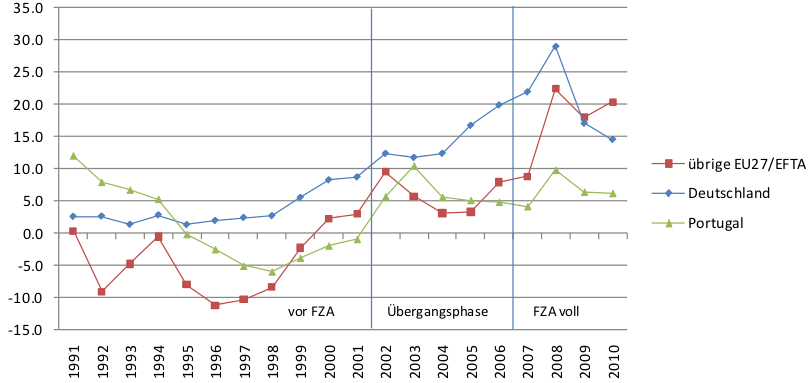
\includegraphics[width=0.9\textwidth]{images/Zuwanderungssaldo_Bericht_2.png}
%	\end{center}
%	\caption{Verlauf der Zuwanderung nach Herkunftsländern in Tausend \cite[S. 18]{ADMIN:Bericht}}
%	\label{fig:zuwanderungsaldi}
%\end{figure*}

